%!TEX encoding = UTF-8 Unicode
%
% Estrutura da analise: 
%     - Summary
%     - How records? How determines the affected?
%     - How removes the effects?
%     - Does it perform replay? How? Of What?
%     - Extra characteristics
%     - Analyze/comments
%
\subsection{Recovery at Operating System Level}
\label{sec:recovery_os}

In this section, we present the main intrusion recovery proposals for operating systems. First, we present the proposal that introduced the main dependencies for operating systems. Then, we present two intrusion recovery systems that use dependency rules and tainting propagation via replay, respectively. Finally, we present proposals to recover from intrusions in computing clusters, virtual machines and network file systems.\\

\textbf{BackTracker \cite{backtracker}:} Backtracker proposes a tainting algorithm to track intrusions. It does not perform any proactive task to remove or recover from intrusions but provides a set of rules for intrusion recovery in operating systems.

Backtracker proposes a tainting algorithm that does tainting analysis offline, after attack detection, as follows. First a graph is initialized with an initial set of compromised processes or files, $D_{tainted}$, identified by the administrator. Then, Backtracker reads the log of system calls from the most recent entry until the intrusion moment. For each process, if it depends on a file or process currently present in the graph then the remaining objects dependent from the process are also added to the graph. The result is a dependency graph (Fig. \ref{fig:graph}) with the objects, including $D_{intrusion}$, which the compromised objects depend from. The following dependency rules establish the graph edges:

\begin{itemize}
  \item \textit{Dependencies process-process:}
  \begin{itemize}
    \item \textit{Process depends on its parent process}: Processes forked from tainted parents are tainted.
    \item \textit{Thread depends on other threads}: Clone system calls to create new threads establish bi-directional dependences since threads share the same address space. Algorithms to taint memory addresses \cite{bezoar} have a significant overhead. Signaling communication between processes also establish dependencies.
  \end{itemize}
  \item \textit{Dependencies process-file:}
  \begin{itemize}
    \item \textit{File depends on Process:} If the process writes the file.
    \item \textit{Process depends on File:} If the process reads the file. 
  \end{itemize}
  
  \item \textit{Dependencies process-filename:}
  \begin{itemize}
    \item \textit{Process depends on filename:} If the process issues any system call that includes the filename, e.g., open, create, link, mkdir, rename, stat, chmod. The process is also dependent of all parent directories of file.
    \item \textit{Filename depends on process:} If any system call modifies the filename, e.g., create, link, unlink, rename.
    \item \textit{Process depends on directory:} If the process reads one directory then it depends on every all filenames on directory.
  \end{itemize}
\end{itemize}

\begin{figure}
  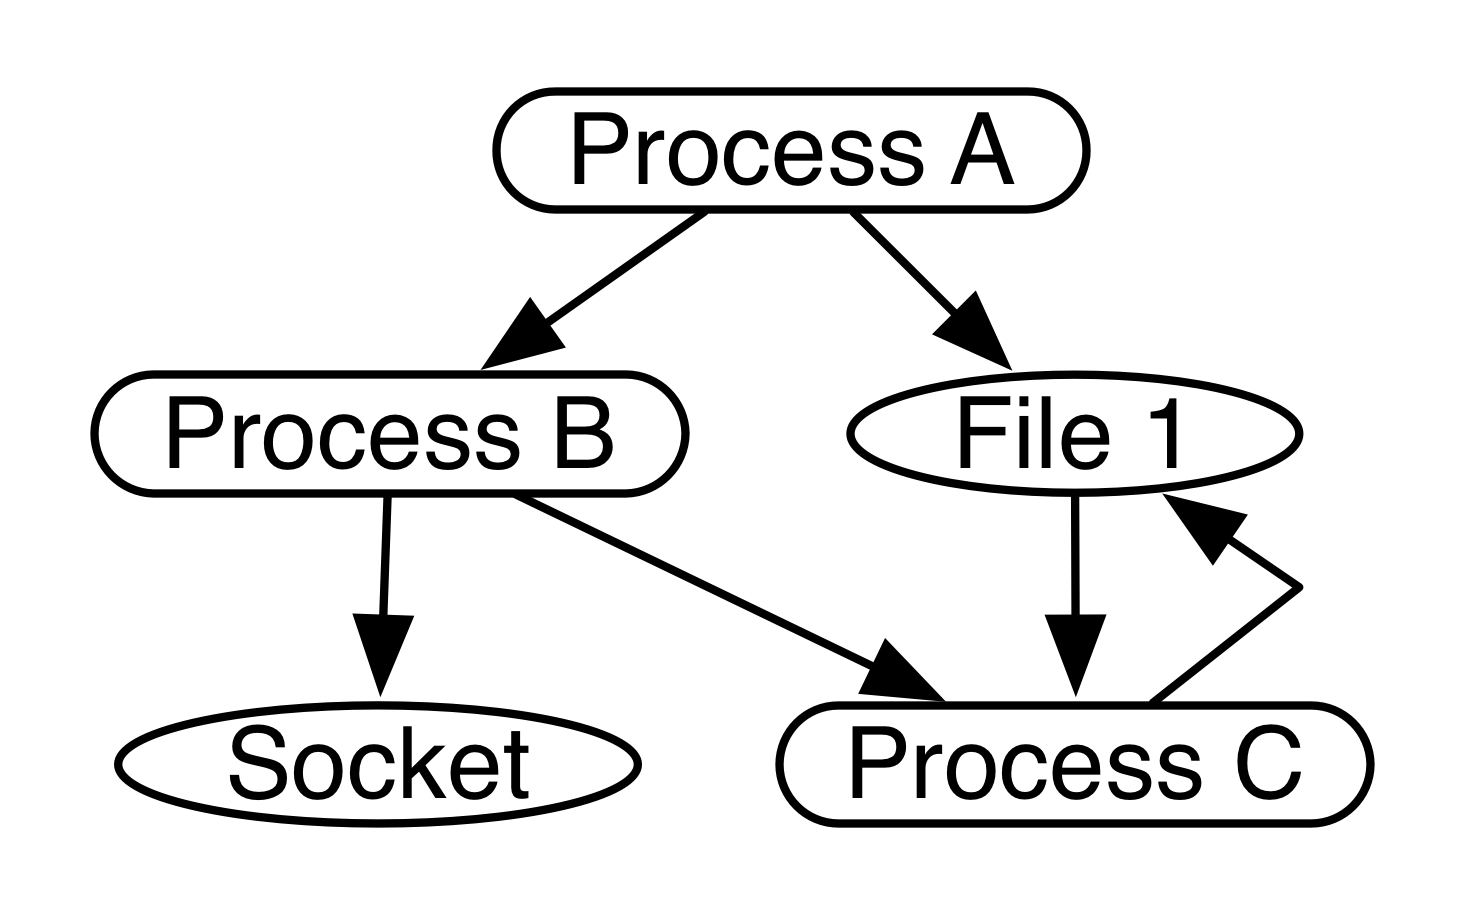
\includegraphics[height=30mm]{images/depGraph}
  \centering
  \caption{Dependency graph generated by BackTracker}
  \label{fig:graph}
\end{figure}

Objects shared between many processes, e.g., \textit{/tmp/} or \textit{/var/run/utmp} are likely to produce false dependencies leading to false positives. Therefore, Backtracker proposes a \textit{white-list} filter that ignores common shared files. However, this technique relies in the administrator knowledge. More, it generates false negatives because it allows the attackers to hide their actions in objects that belong to the white-list. \\


\textbf{Taser \cite{taser}:} Taser removes the intrusion effects from the file system used by the operating system. To do that, it loads a previous version of each tainted file, $D_{tainted}$, from a file-system snapshot, $D_{snapshot}(t)$. Then, to recover the tainted objects, it replays the legitimate modification actions of each tainted object since the snapshot instant $t$.

%record phase
Taser relies on Forensix \cite{forensix} to audit the system actions during the record phase. Forensix logs the names and arguments of every system call related to process management, file system operations and networking. In order to determine the intrusion effects, Taser builds a \textit{object dependency graph} using a set of rules similar to the rules of Backtracker \cite{backtracker}. The object definition encompass files, sockets and processes. Since these rules result in a large number of false dependencies, which mark legitimate objects as \textit{tainted}, Taser provides not only a white list mechanism but also establishes optimistic policies that ignore some dependencies. However, attackers can leverage these optimistic policies to penetrate the operating system.

%How it determines the affected elements?
The recovery phase is started with a set of tainted objects provided by an administrator or an IDS. The provided set of objects can either be the source or the result of an attack. In the latter case, Taser, like Backtracker \cite{backtracker}, transverses the dependency graph in reverse causality order to identify the set of attack source objects, $D_{intrusion}$, which compromised the provided objects. After, at \textit{propagation phase}, Taser transverses the dependency graph from the source objects of the attack, $D_{intrusion}$, to the current moment, adding all tainted objects to the set $D_{tainted}$.

%how it removes
Taser removes the intrusion effects loading a previous version of the tainted objects from a file-system snapshot, $D_{snapshot}(t)$. Then, to recover a coherent state, Taser performs \textit{selective replay}, i.e., it replays, sequentially, the legitimate write operations of the tainted files since the snapshot. Non-tainted files remain unchanged. Since Taser does not checkpoint the state of processes nether the input of each system call, the system must be restarted to remove the current non-persistent states and processes must be replayed from the beginning to load their non-persistent state and perform their system calls with the correct state. This issue has a significant overhead specially for long-run processes as web servers.

 
%does it replays? analyze
Taser does not update the objects originally dependent from tainted objects. In other words, the replay process only recovers a consistent state for the originally tainted objects. Therefore, Taser ignores the set of actions that read the modified version of the tainted files and have a different execution and output. This problem is addressed in \cite{Shafique2006}. More, Taser uses rules to determine the affected files and remove their effects, so it can mistakenly mark legitimate operations as tainted and induce to legitimate data losses.\\



\textbf{RETRO \cite{retro}:} RETRO provides the capability of removing files affected by a set of identified attacking actions. It restores the corrupted files to a previously version using a file system snapshot and then performs selective replay using \textit{taint propagation via replay}. 

%Record Phase:
During the record phase, the kernel module of RETRO creates periodic snapshots of the file system. RETRO logs the input and the output objects of each system call and their associated process. The object definition encompasses not only files and directories but also TCP sessions and the operating system console (tty). The dependencies are established per system call instead of per process. Therefore, the graph is finer-grained than the graph of Backtracker \cite{backtracker} and reduces the number of false positives.

%remove
During the recovery phase, RETRO requires the administrator to identify $A_{intrusion}$, processes, system calls or $D_{intrusion}$ objects which caused the intrusion. First, it removes the malicious system calls from the graph. Then it performs \textit{taint propagation via replay}. To do so, it loads a previous version, from a snapshot, of the objects in $D_{intrusion}$. Then, the system calls, which are dependent from the restored objects, are replayed and their output objects are updated. The forward system calls, which depend from the updated objects, are also replayed while their inputs are different from the original execution. The propagation is done thought the output of system calls with different execution. The recovery process terminates when propagation stops. Since RETRO records the system call input, it can replay processes with system call granularity instead of process granularity, so the replay process may stop earlier. However, this mechanisms forces that the process re-execution has the same sequence of system calls as its original execution. Therefore, the process source code nether its sequence of actions can not change. 

%external dependencies
Since RETRO replays the processes, the external state may change. External changes are manifested through operating system console and network objects. RETRO emails the administrator with the textual difference between the original and recovery outputs. Later work of the same authors, \textit{Dare} \cite{dare}, extends RETRO to recover from intrusions in distributed systems. It adds the dependencies through sockets. The machines involved in a network session add socket objects to the dependency graph. Network protocol, source and destination IP and ports and one ID, which are exchanged in every package during the connection, globally identify each socket object. The recovery phase in Dare is similar RETRO except on network system calls handlers. Compromised network sessions must be replayed since their input depends on destination server. Therefore, prior to invoke the system call for network session establishment, Dare invokes a remote method at receiver Dare daemon to rollback the network session. The receiver rollback the dependent objects to the version before session establishment and replays their dependencies. The remote method response includes the re-execution output. The local system updates the system call output. The re-execution is propagated if this output is different. 

%Analyse
The efficiency of RETRO comes from avoiding to replay the actions if their input remains equal. However, the invoked system call must remain the same. Therefore, RETRO does not support a distinct process execution. RETRO requires human intervention to solve external inconsistencies. Dare solves it but it is limited to clusters where every operating system runs a Dare and RETRO daemon. RETRO can not recover from an intrusion whose log files have been garbage collected or deleted. Dare supports distributed re-execution but, as RETRO, the affected machines must be offline because its propagation algorithm shutdown the service during the repair phase. \\



\textbf{Bezoar \cite{bezoar}:} Bezoar proposes a rewind based approach to recover from attacks coming from the network in virtual machines (VM). The snapshot is performed by VM forking using copy-on-write. This snapshot technique encompasses the entire system: processes and kernel spaces, resources, file system, virtual memory, CPU registers, virtual hard disk and memory of all virtual external devices. Bezoar tracks how the data from network connections propagates in memory. During the recovery phase, the administrator identifies the network connections used by the attackers. Bezoar removes the intrusion effects using rewind. It loads a previous VM snapshot and it replays the system execution ignoring all network packets from the identified malicious sources. 

The recovery process using rewind is longer than RETRO or Taser because all external requests are replayed but supports distinct process execution. Bezoar requires system outage during the replay phase and does not provide any external consistency warranties.\\


\textbf{Repairable File System (RFS) \cite{rfs}:} RFS is designed to recover compromised network file systems. The novelty in RFS comparing with the previously introduced systems is its client-server architecture. RFS includes a client and a server module for a network file system (NFS).

The client module tracks the system calls using ExecRecorder \cite{Oliveira2006} and establishes the dependence between processes and NFS requests. Every request to the NFS server is marked with a request ID and the client ID. At server side, the request interceptor logs all requests sent by clients to update files. Requests are ordered in per-filename queues. They are processed locally and write operations are mirrored to external server asynchronously after reply. The external server keeps all file versions. 

During the recovery phase, the server defines the contaminated processes using the client logs. A process is contaminated if it matches a set of rules similar to Backtracker \cite{backtracker}. RFS adds the concept of contaminated file and contaminated file block. If a file is contaminated, all its blocks are contaminated. The reverse is not true, i.e., processes remains non-contaminated if they read a correct block from a contaminated file. RFS uses the version server to rollback only the affected files. \\



\textbf{Summary:} Dependencies at the operating system level are established by rules based on BackTracker \cite{backtracker}. These rules are vulnerable to false positives and false negatives. While Taser \cite{taser} and RFS \cite{rfs} recover from intrusions removing the effects only in corrupted files, RETRO \cite{retro} removes the values written by $A_{intrusion}$ and replays the forward system calls while their input changes. If $A_{intrusion}$ is identified properly, then RETRO does not have false positives.

The operating system level services are vulnerable to attacks inside kernel because they only audit the system calls. Attackers can compromise the recovery system because the log daemons are installed in the machine where attacks are performed. The recovery guarantees are limited by the system administrator capability to detect the attack and pinpoint the intrusion source. Administrators must avoid false positives to prevent legitimate data losses. However, remove false dependencies can take a while because the low abstraction level creates bigger dependency graphs and logs.



